\chapter{Connector Pinouts}
\section{Full-Duplex RS-485 Connection (8p8c Female Modular Jacks)}
\begin{center}
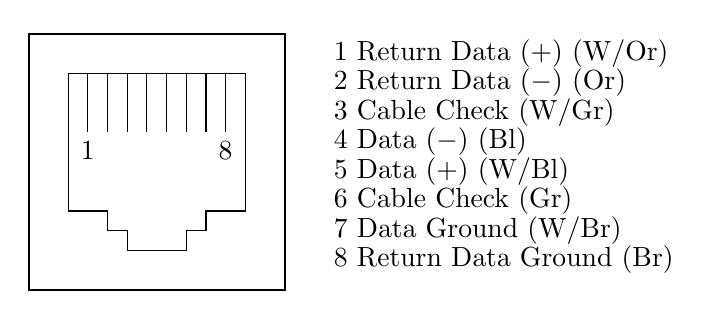
\begin{tikzpicture}[scale=.25]
	\draw [thick] (0,0) -- (0,13) -- (13,13) -- (13,0) -- cycle;
	\draw (2,11) -- (11,11) -- (11,4) -- (9,4) -- (9,3) -- (8,3) -- (8,2) -- (5,2) -- (5,3) -- (4,3) -- (4,4) -- (2,4) -- cycle;
	\foreach \x in {3, 4, 5, 6, 7, 8, 9, 10} {
		\draw (\x,11) -- (\x,8);
	}
	\node [below] at (3,8) {1};
	\node [below] at (10,8) {8};
	\node [right] at (15,12) {\strut 1 Return Data ($+$) (W/Or)};
	\node [right] at (15,10.5) {\strut 2 Return Data ($-$) (Or)};
	\node [right] at (15,9) {\strut 3 Cable Check (W/Gr)};
	\node [right] at (15,7.5)  {\strut 4 Data ($-$) (Bl)};
	\node [right] at (15,6)  {\strut 5 Data ($+$) (W/Bl)};
	\node [right] at (15,4.5)  {\strut 6 Cable Check (Gr)};
	\node [right] at (15,3)  {\strut 7 Data Ground (W/Br)};
	\node [right] at (15,1.5)  {\strut 8 Return Data Ground (Br)};
\end{tikzpicture}
\end{center}

\section{Half-Duplex RS-485 Connection (6p6c Female Modular Jacks)}
\begin{center}
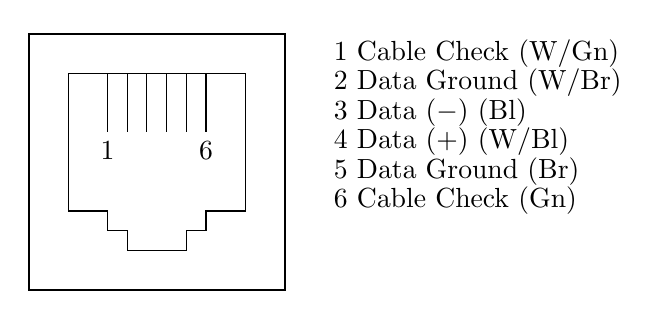
\begin{tikzpicture}[scale=.25]
	\draw [thick] (0,0) -- (0,13) -- (13,13) -- (13,0) -- cycle;
	\draw (2,11) -- (11,11) -- (11,4) -- (9,4) -- (9,3) -- (8,3) -- (8,2) -- (5,2) -- (5,3) -- (4,3) -- (4,4) -- (2,4) -- cycle;
	\foreach \x in {4, 5, 6, 7, 8, 9} {
		\draw (\x,11) -- (\x,8);
	}
	\node [below] at (4,8) {1};
	\node [below] at (9,8) {6};
	\node [right] at (15,12) {\strut 1 Cable Check (W/Gn)};
	\node [right] at (15,10.5) {\strut 2 Data Ground (W/Br)};
	\node [right] at (15,9) {\strut 3 Data ($-$) (Bl)};
	\node [right] at (15,7.5)  {\strut 4 Data ($+$) (W/Bl)};
	\node [right] at (15,6)  {\strut 5 Data Ground (Br)};
	\node [right] at (15,4.5)  {\strut 6 Cable Check (Gn)};
%	\node [right] at (15,3)  {\strut 7 Data Ground};
%	\node [right] at (15,1.5)  {\strut 8 Return Data Ground};
\end{tikzpicture}
\end{center}
%Note that the jacks are labeled ``\mc{IN}'' and ``\mc{OUT/THRU}'' on the board.  This is intended to remind the user
%that these are daisy-chained connections with a signal coming ``in'' to the board on one wire, and on ``through'' to
%the next board in the circuit.% (or ``out'' back to the host PC in the case of responses to query commands).  
%These
%names also mirror the naming conventions used with \acronym{DMX} equipment. 
%
%Electrically, however, the RS-485 serial ``network'' is a single bus running from the host PC to the last Lumos
%controller.  Each controller ``taps'' into the line as it goes by.  This means that, labeling notwithstanding,
%the ``\mc{IN}'' and ``\mc{OUT/THRU}'' jacks are in fact completely identical and interchangeable.
%
%The ``cable check'' lines are simply passed through the Lumos board from input to output, with the expectation that
%the terminator will connect them together.  These lines are not used by Lumos boards at all.  They are provided as
%a convenient way for the host PC interface to verify cable continuity by sending a voltage down one pin all
%the way to the terminator and back on the other pin.  This helps warn the user if a cable becomes disconnected.
%The Lumos front panel circuit board is one example of a circuit which makes use of this feature.
%
%The two grounds on pins 7 and 8 are actually shorted together and connected to the common signal ground
%on the Lumos board.
%
%If connecting a Lumos board to a \acronym{DMX} controller, an adapter cable is needed to connect the
%\acronym{DMX} \acronym{DIN} plug to the 8-pin modular plug used on the Lumos board.  A typical adapter is wired as shown in Table~\ref{tbl:dmx8p}, but check your equipment in case it is different.
%\begin{table}
% \begin{center}
%  \begin{tabular}{ccc}\toprule
%	\bfseries Signal &
%	\bfseries \acronym{DMX} \acronym{DIN} Connector &
%	\bfseries Lumos Modular Connector\\\midrule
%	Ground & 1 & 7, 8 \\
%	Data ($-$) & 2 & 4 \\
%	Data ($+$) & 3 & 5 \\\bottomrule
%  \end{tabular}
%  \caption{Typical Wiring Arrangement to Adapt \acronym{DMX} to Lumos\label{tbl:dmx8p}}
% \end{center}
%\end{table}
%
%\newpage
%
%\section{RS-485 Terminator (8p8c Male Plug)}
%The terminator plug consists of a pair of 120\,$\Omega$ resistors.  One is connected across pins 1--2, and the other
%across pins 4--5.  This provides the proper line termination at the end of the RS-485 chain.  A terminator must
%be plugged in to each end of the chain (but note that often the PC's RS-485 adaptor contains a built-in terminator).
%
%To enable the cable check feature to work, pins 3 and 6 must also be shorted together.
%
%The schematic diagram for the terminator is included below.  Often, the resistors are mounted to a small circuit
%board which fits inside the modular plug, making a self-contained terminator plug.\label{sch:terminator}
%\begin{center}
%	\begin{circuitikz}
%		\draw (0,0) -- (1,0) -- (1,4.5) -- (0,4.5) -- cycle;
%		\node at (.5,.5) {8};
%		\node at (.5,1) {7};
%		\node at (.5,1.5) {6};
%		\node at (.5,2) {5};
%		\node at (.5,2.5) {4};
%		\node at (.5,3) {3};
%		\node at (.5,3.5) {2};
%		\node at (.5,4) {1};
%		\draw (1,4) to[R, l=120\,$\Omega$] (3,4);
%		\draw (3,4) -- (3,3.5) -- (1,3.5);
%		\draw (1,2.5) to[R] (3,2.5);
%		\draw (3,2.5) -- (3,2.0) -- (1,2.0);
%		\draw (1,3) -- (4,3) -- (4,1.5) -- (1,1.5);
%	\end{circuitikz}
%\end{center}
%
%\section{RS-232 Serial Connection (9-pin Female DE-9 Jack)}
%\begin{center}
%	\begin{tikzpicture}[scale=.25]
%		\draw [thick] (0,7) -- (12,7) -- (10,3) -- (2,3) -- cycle;
%		\foreach \x in {2, 4, 6, 8, 10} {
%			\draw (\x, 6) circle (.5);
%		}
%		\foreach \x in {3, 5, 7, 9} {
%			\draw (\x, 4) circle (.5);
%		}
%		\node [above] at (10,7) {1};
%		\node [above] at (2,7) {5};
%		\node [below] at (3,3) {9};
%		\node [below] at (9,3) {6};
%		\node [right] at (14,7) {2 Receive Data\strut};
%		\node [right] at (14,5.5) {3 Transmit Data\strut};
%		\node [right] at (14, 4) {4 Data Terminal Ready\strut};
%		\node [right] at (14, 2.5) {5 Signal Ground\strut};
%		\node [right] at (30, 7) {6 Data Set Ready\strut};
%		\node [right] at (30, 5.5) {7 Request to Send\strut};
%		\node [right] at (30, 4) {8 Clear to Send\strut};
%	\end{tikzpicture}
%\end{center}
%For Lumos boards configured to use RS-232 serial connections to a host PC, a standard 9-pin connector is used,
%with the Lumos board wired as a \acronym{DCE} device.
%
%On the Lumos board, Data Terminal Ready (\acronym{DTR}) and Data Set Ready (\acronym{DSR}) on pins 4 and 6 are shorted
%together, as are Request to Send (\acronym{RTS}) and Clear to Send (\acronym{CTS}) on pins 7 and 8.  This should satisfy
%most communications software which expects to see these signals present, although the Lumos board itself does not
%perform any hardware or software handshaking.
%
%Receive Data (\acronym{RxD}) and Transmit Data (\acronym{TxD}) are named from the point of view of the \acronym{DTE} (host
%PC), so \acronym{TxD} is the wire which carries data from the host PC to the Lumos board.
%
%\section{Sensor Input Terminals (J16)}
%\begin{center}
%	\begin{tikzpicture}[scale=.5]
%		\draw [thick] (.5,.5) -- (5.5,.5) -- (5.5,1.5) -- (.5,1.5) -- cycle;
%		\foreach \x in {1, 2, 3, 4, 5} {
%			\draw (\x,1) circle (.4);
%		}
%		\draw [thick] (4.5, .5) -- (4.5, 1.5);
%		\node [above] at (1,1.5) {$\overline{\hbox{A}}$};
%		\node [above] at (2,1.5) {$\overline{\hbox{B}}$};
%		\node [above] at (3,1.5) {$\overline{\hbox{C}}$};
%		\node [above] at (4,1.5) {$\overline{\hbox{D}}$};
%		\node [above right] at (4.5,1.5) {$\overline{\hbox{PWR CTL}}$};
%		\node [left] at (.5,1) {J16};
%		\node [right] at (5.5,1) {J9};
%		\draw (4,.4) -- (3.8,.1) -- (4.2,.1) -- cycle;
%		\draw (5,.4) -- (4.8,.1) -- (5.2,.1) -- cycle;
%	\end{tikzpicture}
%\end{center}
%If the Lumos controller is built to accommodate one or more sensor inputs, a set of terminals will be installed
%at J16, next to the $\overline{\hbox{\mc{PWR CTL}}}$ output at J9.  These are labeled from left to right (as the board
%is viewed right-side-up from the front) as 
%$\overline{\hbox{\mc{A}}}$,
%$\overline{\hbox{\mc{B}}}$,
%$\overline{\hbox{\mc{C}}}$, 
%and
%$\overline{\hbox{\mc{D}}}$.
%It is important to note that the board's circuitry must be configured for certain inputs to be enabled
%at the time the board is built, and that the board must be configured (using software) to recognize those
%inputs, before they will be usable.
%
%Each input accepts a \acronym{TTL}-level signal.  The lines are pulled up to +5\,V internally.  The board
%can be configured in software to react to the inputs as active-high or active-low.
%
%\section{Logic Output Terminals (J18)}
%\begin{center}
%	\begin{tikzpicture}[scale=.5]
%		\draw [thick] (.5,.5) -- (5.5,.5) -- (5.5,1.5) -- (.5,1.5) -- cycle;
%		\foreach \x in {1, 2, 3, 4, 5} {
%			\draw (\x,1) circle (.4);
%		}
%		\node [above] at (1,1.5) {0};
%		\node [above] at (2,1.5) {1};
%		\node [above] at (3,1.5) {2};
%		\node [above] at (4,1.5) {3};
%		\node [above right] at (4.5,1.5) {GND};
%		\node [left] at (.5,1) {J18};
%	\end{tikzpicture}
%\end{center}
%For experimental use, \acronym{TTL}-level outputs for the first four channels are available on J18.  These
%are active-low outputs, where a ``low'' (0) state indicates that the output should be on, and a ``high''
%(1) state means that the output should be off.  Note that if an output is at a dimmer level other than
%fully on or fully off, the signal will pulse with a duty cycle corresponding to the dimmer level as illustrated
%in Figure~\ref{fig:dutycycle}.
%
%%15
%%14...........
%%13------------
%%12............
%%11
%%10...........
%% 9------------
%% 8............
%% 7
%% 6...........
%% 5------------
%% 4............
%% 3
%% 2...........
%% 1------------
%% 0............
%
%\input dutycycle
%
%\section{ICSP Header (J11)}
%\begin{center}
%	\begin{tikzpicture}[scale=.5]
%		\draw [line width=10] (.6,1)--(5.4,1);
%		\foreach \x in {1, 2, 3, 4, 5} {
%			\foreach \y in {1} {
%				\draw [fill=white] (\x-.2,\y-.2) -- (\x-.2,\y+.2) -- (\x+.2,\y+.2) -- (\x+.2,\y-.2) -- cycle;
%			}
%		}
%		\draw (5.5,1) -- (6,1.25) -- (6,0.75) -- cycle;
%		\node [above] at (1,1.5) {5};
%		\node [above] at (2,1.5) {4};
%		\node [above] at (3,1.5) {3};
%		\node [above] at (4,1.5) {2};
%		\node [above] at (5,1.5) {1};
%		\node [right] at (7, 3.0) {1 $\hbox{V}_{\hbox{\footnotesize DD}}$ (+5\,V)};
%		\node [right] at (7, 2.0) {2 $\hbox{V}_{\hbox{\footnotesize SS}}$ (Ground)};
%		\node [right] at (7, 1.0) {3 $\hbox{V}_{\hbox{\footnotesize PP}}/\overline{\hbox{\mc{MCLR}}}/\overline{\hbox{\mc{RESET}}}$};
%		\node [right] at (15, 3.0) {4 PGD$/\overline{\hbox{\mc{PWR CTL}}}$};
%		\node [right] at (15, 2.0) {5 PGC$/\overline{\hbox{\mc{OPTION}}}$};
%	\end{tikzpicture}
%\end{center}
%
%This header is used for reprogramming a new firmware image onto the microcontroller chip.  Be sure to check the pinout
%used by your programmer before connecting it to this port.  It may be different!
%
%During normal operations, this header may also be used to connect off-board buttons for the reset and option functions.  These
%buttons should be normally open, but connect their respective pins to ground when pushed. 
%Note that the $\overline{\hbox{\mc{PWR CTL}}}$ output is also present on pin~4 of J11 in addition to its normal
%terminal at J9.
%
%
%\section{Voltage Select Headers (J6--J8, J17)}\label{sec:voltagesw}
%\begin{center}
%	\begin{tikzpicture}[scale=.5]
%		%\draw [line width=10] (.6,1)--(4.4,1);
%		\draw [line width=10] (1,.6)--(1,4.4);
%		\draw [line width=10] (5,.6)--(5,4.4);
%		\foreach \y in {1, 2, 3, 4} {
%			\foreach \x in {1, 5} {
%				\draw [fill=white] (\x-.2,\y-.2) -- (\x-.2,\y+.2) -- (\x+.2,\y+.2) -- (\x+.2,\y-.2) -- cycle;
%			}
%		}
%		\node [above] at (1,4.4) {J17};
%		\node [above] at (5,4.4) {J6--J8};
%		\node [left] at (.8,1) {VRO};
%		\node [left] at (.8,2) {+O};
%		\node [left] at (.8,3) {+I};
%		\node [left] at (.8,4) {VRI};
%		\node [left] at (4.8,1) {VRI};
%		\node [left] at (4.8,2) {+I};
%		\node [left] at (4.8,3) {+O};
%		\node [left] at (4.8,4) {VRO};
%
%		\node [right] at (7, 4) {+I: Positive voltage in from power supply};
%		\node [right] at (7, 3) {+O: Positive voltage out to circuit};
%		\node [right] at (7, 2) {VRI: Input to voltage regulator};
%		\node [right] at (7, 1) {VRO: Output from voltage regulator};
%	\end{tikzpicture}
%\end{center}
%J6--J8 are used to select the input voltage supplied to the power control blocks for channels 0--7, 8--15, and 16--23
%respectively.  Likewise, J17 selects the input voltage supplied to the logic portion of the board.  Although the pinouts
%are mirrored between J17 and the others, their operation is the same.  If a regulated +5\,V supply is employed, there is no
%need for the on-board regulator (and in fact it can't function properly unless its input is at least +8\,V), so a jumper
%is placed across the middle two pins (connecting +I and +O), bypassing the voltage regulator entirely.  \emph{In this 
%case, it is critically important that the input voltage be a clean, regulated +5\,V supply.  If this voltage is exceeded,
%permanent damage to the Lumos board will result!}
%
%If +8\,V to +24\,V is attached to an input, the corresponding jumper block needs jumpers installed into the outer two pins,
%connecting +I to VRI and +O to VRO.  This routes the incoming power through the voltage regulator.
%
%\input{voltagedpdt}
%
%\section{Relay Control Connection (26-pin Male IDC Header)}
%%
%%   . . . . . . . . . . . . .
%%   . . . . . . . . . . . . .
%%
%\begin{center}
%	\begin{tikzpicture}[scale=.25]
%		\foreach \x in {1, 2, 3, 4, 5, 6, 7, 8, 9, 10, 11, 12, 13} {
%			\foreach \y in {1, 2} {
%				\draw (\x-.1,\y-.1) -- (\x-.1,\y+.1) -- (\x+.1,\y+.1) -- (\x+.1,\y-.1) -- cycle;
%			}
%		}
%		%\draw         (.4,.4) -- (.4,2.6) -- (13.6,2.6) -- (13.6,.4) -- (.4,.4);
%		\draw         (.4,.4) -- (.4,2.6) -- (13.6,2.6) -- (13.6,.4) -- (8,.4) -- (8,.2) -- (6,.2) -- (6,.4) -- cycle;
%		\draw [thick] (.2,.2) -- (.2,2.8) -- (13.8,2.8) -- (13.8,.2) -- cycle;
%		\node [below] at (1,0) {\strut1};
%		\node [above] at (1,3) {\strut2};
%%		\node [below] at (2,0) {\strut3};
%%		\node [above] at (2,3) {\strut4};
%		\node [below] at (3.5,0) {\strut$\cdots$};
%		\node [above] at (3.5,3) {\strut$\cdots$};
%		\node [below] at (13,0) {\strut 25};
%		\node [above] at (13,3) {\strut 26};
%	\end{tikzpicture}
%\end{center}
%For Lumos controllers built as ``dumb'' relay boards with no built-in logic control of their own, a 26-pin 
%\acronym{IDC} ribbon cable header is installed at J14.  This is used to connect the relays to the controlling circuit (e.g.,
%a Lumos 48-channel controller).  The pinout of this header is:
%\begin{center}
%	\begin{tabular}{rl|rl|rl|rl}
%1&$\overline{\hbox{\mc{SSR23}}}$&8&$\overline{\hbox{\mc{SSR3}}}$&15&Gnd                           &22&$\overline{\hbox{\mc{SSR9}}}$ \\
%2&$\overline{\hbox{\mc{SSR0}}}$&9&$\overline{\hbox{\mc{SSR19}}}$&16&+5\,V                         &23&$\overline{\hbox{\mc{SSR13}}}$ \\
%3&$\overline{\hbox{\mc{SSR22}}}$&10&$\overline{\hbox{\mc{SSR4}}}$&17&$\overline{\hbox{\mc{SSR16}}}$&24&$\overline{\hbox{\mc{SSR10}}}$ \\
%4&$\overline{\hbox{\mc{SSR1}}}$&11&$\overline{\hbox{\mc{SSR18}}}$&18&$\overline{\hbox{\mc{SSR7}}}$&25&$\overline{\hbox{\mc{SSR12}}}$\\
%5&$\overline{\hbox{\mc{SSR21}}}$&12&$\overline{\hbox{\mc{SSR5}}}$&19&$\overline{\hbox{\mc{SSR15}}}$&26&$\overline{\hbox{\mc{SSR11}}}$\\
%6&$\overline{\hbox{\mc{SSR2}}}$&13&$\overline{\hbox{\mc{SSR17}}}$&20&$\overline{\hbox{\mc{SSR8}}}$\\
%7&$\overline{\hbox{\mc{SSR20}}}$&14&$\overline{\hbox{\mc{SSR6}}}$&21&$\overline{\hbox{\mc{SSR14}}}$
%	\end{tabular}
%\end{center}
